
\section{Netzwerke}
Netzwerke setzen sich im allgmeinen aus $N$ Knoten (Nodes) zusammen, die über gewichtete Verbindungen (Edges) miteinander Verbunden sind. Besteht zwischen zwei Knoten eine Verbindung in beide Richtungen, so spricht man von einem ungerichteten Netzwerk. Wenn alle Knoten untereinander verbunden sind, so handelt es sich um ein vollständiges Netzwerk (siehe Abbildung \ref{fig:GraphBsp}).

\begin{figure}[t]
	 \centering
	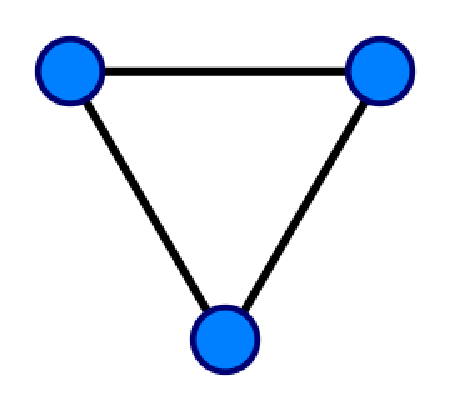
\includegraphics[width=0.3\textwidth]{abb/misc/GraphBsp.eps}
	\caption[Ungerichteres Netzwerk]{Beispiel eines ungerichteten Netzwerks aus drei Knoten, bei dem jeder Knoten mit jedem anderen Verbunden ist.}
	\label{fig:GraphBsp}
\end{figure}


\subsection{Dynamik auf Netzwerken}
Um Prozesse auf Netzwerken zu beschreiben kann man jedem Knoten eine dynamische Variable zuordnen. Die Dynamik wird dann für jeden Knoten über eine Differentialgleichung beschrieben, die die Kopplung an die anderen Knoten enthält. Die allgemeine Form dieser Differentialgleichung ist für ein System ohne Rückkopplung in Gleichung (\ref*{eq:dyneqcommon}) gezeigt.
\begin{align}\label{eq:dyneqcommon}
\overset{\cdot}{\boldsymbol{x}}_i(t)&=\boldsymbol{f}(\boldsymbol{x}_i(t))+\sigma\sum_j A_{ij}\boldsymbol{h}\left(\boldsymbol{x}_j(t)\right)
\\\notag & i=1,...,N
\\\notag & \sigma \text{ allgemeine Kopplungsstärke}
\\\notag & A_{ij}\text{ Kopplungsmatrix}
\\\notag & \boldsymbol{f},\boldsymbol{h}:\mathbb{R}^n\rightarrow\mathbb{R}^n
\end{align}
$\boldsymbol{A}$ ist dabei die Kopplungsmatrix, in der für ein Netzwerk, bei dem die Knoten alle gleich stark an einander koppeln, die Einträge entweder 0 oder 1 sind. Im folgenden werden nur solche Systeme betrachtete, bei denen $\boldsymbol{A}$ symmetrisch ist, das Netzwerk also ungerichtet. Die Abbildung $\boldsymbol{h}$ beschreibt auf welche Art und Weise die Komponenten der Variablen $\boldsymbol{x}_i$ aneinander koppeln. Das Differentialgleichungssystem in (\ref*{eq:dyneqcommon}) lässt sich auch über das Kronecker-Produkt in einer einzigen Gleichung darstellen,
\begin{align}
\overset{\cdot}{\boldsymbol{X}}(t)=\boldsymbol{F}(\boldsymbol{X}(t))+\sigma\boldsymbol{A}\otimes\boldsymbol{H}(\boldsymbol{X}(t))
\end{align}
mit den Definitionen:
\begin{align*}
\boldsymbol{X}=\left(\boldsymbol{x}_1,...,\boldsymbol{x}_N\right)^{\text{T}},
\boldsymbol{F}=\left(\boldsymbol{f}(\boldsymbol{x}_1),...,\boldsymbol{f}(\boldsymbol{x}_N)\right)^{\text{T}},
\boldsymbol{H}=\left(\boldsymbol{h}(\boldsymbol{x}_1),...,\boldsymbol{h}(\boldsymbol{x}_N)\right)^{\text{T}}
\end{align*}

